\chapter{O que é visão computacional e OCR?}

Este capítulo apresenta os conceitos básicos de visão computacional e OCR. Não serão abordados a fundo como ambos funcionam, mas sim para que e onde são utilizados.  

\section{Visão computacional}

A Visão Computacional é um campo de estudo da computação que tem por objetivo tornar possível um computador ver e analisar imagens, extraindo informações úteis de componentes como uma câmera de vídeo, \textit{scanners} e dispositivos semelhantes \cite{computervision}. Em outras palavras, visão computacional tem o objetivo final de usar computadores para emular a visão humana, incluindo a aprendizagem e a capacidade de fazer inferências e tomar decisões baseadas nas entradas fornecidas. Essa área é um ramo que pertence à inteligência artificial, que por sua vez tem o objetivo central de emular a inteligência humana \cite{computervision}. A análise de uma imagem está entre o processamento de imagens e a visão computacional \cite{gonzalez}.

Entre processamento de imagens e visão computacional podem ser encontrados três níveis de processos, respectivamente, baixo-nível, nível-médio e alto-nível. Os processos de baixo-nível envolvem operações primárias, tais como a redução de ruído ou melhoria no contraste de uma imagem. Os processos de nível-médio são operações do tipo segmentação (particionamento da imagem em regiões) ou classificação (reconhecimento dos objetos na imagem). Os processos de alto-nível estão relacionados com as tarefas de cognição associadas com a visão humana \cite{gonzalez}.

Olhando para um grupo de pessoas em um porta-retratos, os seres humanos são capazes de identificar cada pessoa, reconhecer o nome e, através da expressão facial, até mesmo obter conhecimento do comportamento sentimental da pessoa naquele momento. Estudiosos passaram décadas tentando compreender como o sistema visual funciona, e chegaram a bons resultados em certas áreas como reconhecimento de texto. Mas ainda há muito para evoluir como na inteligência artificial de uma forma geral \cite{marr} \cite{palmer}.

Atualmente, com os avanços em visão computacional, pode-se identificar com alta probabilidade pessoas em meio a um cenário complexo, ou seja, que contenha diversos outros objetos incluídos, como árvores, carros, animais e outros, e dar-lhes os respectivos nomes. A \autoref{fig:recPessoas} ilustra a detecção de seis pessoas dentro de um barco, e a \autoref{fig:recCenario} ilustra um sistema capaz de reconhecer uma pessoa em meio a um cenário que contém árvores, prédio, cadeiras e outros objetos, circulando a cabeça, os braços, mãos e pernas. Entretanto, não é possível dizer ainda que visão computacional consegue emular a visão de uma criança de dois anos, devido principalmente, ao grande número de incógnitas para poucos dados \cite{caap}.

\begin{figure}[htb]
 \label{fig:reconhecimento}
 \centering
  \begin{minipage}{0.48\textwidth}
    \centering
    \caption{Reconhecimento de seis pessoas em um barco} \label{fig:recPessoas}
    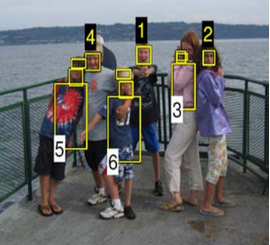
\includegraphics[width=.95\textwidth]{figuras/f1c2.png}
    \legend{Fonte:\citeonline{caap}}
  \end{minipage}
  \hfill
  \begin{minipage}{0.48\textwidth}
    \centering
    \caption{Reconhecendo e circulando pessoa em meio a cenário complexo} \label{fig:recCenario}
    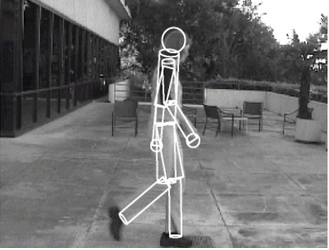
\includegraphics[width=.95\textwidth]{figuras/f2c2.png}
    \legend{Fonte: \citeonline{caap}}
  \end{minipage}
\end{figure}


%\begin{figure}[htbp]
%\caption{\label{fig:recPessoas} Reconhecimento de seis pessoas em um barco}
%\begin{center}
%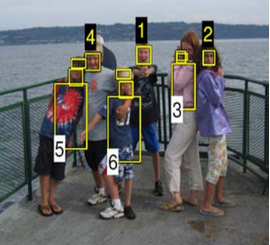
\includegraphics[width=.5\textwidth]{figuras/f1c2.png}
%\end{center}
%\legend{Fonte:\citeonline{caap}}
%\end{figure}

%\begin{figure}[htbp]
%\caption{\label{fig:recCenario}Reconhecendo e circulando pessoa em meio a cenário complexo}
%\begin{center}
%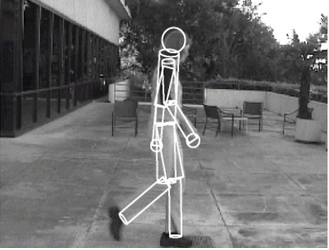
\includegraphics[width=.5\textwidth]{figuras/f2c2.png}
%\end{center}
%\legend{Fonte:\citeonline{caap}}
%\end{figure}

A visão computacional está sendo utilizada hoje em diversos meios, como \cite{caap}:


\begin{alineas}
\item no reconhecimento óptico de caracteres (OCR) aplicado a outros sistemas;
\item em sistemas de inspeção da máquina, em que são realizadas inspeções para garantia de qualidade, medindo as tolerâncias das asas de aviões, ou procurando defeitos em peças fundidas de aço, utilizando raios-X;
\item em construção de modelos 3D (fotogrametria) de forma totalmente automatizada a partir de fotografias aéreas utilizadas em sistemas como o Bing Maps \cite{bingmaps};
\item na radiologia é utilizado para registrar imagens pré-operatórias e intra-operatórias, ou na realização de estudos de longo prazo da morfologia do cérebro das pessoas à medida que envelhecem;
\item na área de segurança automotiva, tem-se o sistema de detecção de obstáculos inesperados, como pedestres na rua;
\item em jogos de movimentos, fundindo imagens geradas por computador com cenas de ação ao vivo por rastreamento de pontos característicos no vídeo fonte. Tais técnicas são amplamente utilizadas em Hollywood (por exemplo, filme Jurassic Park) \cite{robinandzafar};
\item em autenticação visual com o uso da \textit{webcan} para autenticação de usuário;
\item em câmeras digitais através da detecção facial, auxiliando a câmera digital a focar na região correta;
\item nos bancos, onde pode-se fazer autenticação por biometria, sendo as medidas biometricas a chave de segurança; 
\end{alineas}

\section{Reconhecimento ótico de caracteres}

Reconhecimento ótico de caracteres é uma das áreas que envolve visão computacional como analisado anteriormente. \citeonline{ocr} faz a seguinte definição de OCR:
\begin{citacao}	
O processo de reconhecimento óptico de caracteres (OCR) envolve o uso de sistemas de imagem e computadores para converter texto manuscrito ou impresso em texto que a máquina é capaz de codificar e reconhecer. OCR possui muitos usos, como a simplificação de entrada de dados, reconhecimento de placa de licença de veículos, e disponibilização de cópias editáveis de documentos impressos \cite{ocr}.
\end{citacao}
De maneira comercial, alguns sistemas OCRs começaram a surgir por volta de 1960, porém esses sistemas possuíam muitas limitações. Essa foi considerada a primeira geração de sistemas OCR. A segunda geração surgiu próxima do início de 1970, onde os sistemas OCRs já eram capazes de maneira singela, de reconhecer cartas escritas a mão. Pouco tempo depois, surge a terceira geração, dando resultados mais precisos sendo usados em \textit{scanners} \cite{eikvil1993optical}. Os estudos estão continuamente sendo feitos desde então buscando melhorias, mas não há registros muito relevantes, nem mesmo nomeações oficiais de novas gerações. 

Há dois tipos de sistemas que podem ser encontrados de forma geral com o uso de OCRs: sistemas de reconhecimento de caracteres offline (OffOCR) e sistemas de reconhecimento de caracteres online (OnOCR). Ambos são muito utilizados e sua diferença principal é bem clara. Os sistemas OffOCRs fazem o reconhecimento do texto depois de ser impresso ou escrito a mão, necessitando apenas iniciar um processo de escaneamento para então o reconhecimento propriamente dito. Já os sistemas OnOCRs fazem o reconhecimento ainda enquanto o texto está sendo produzido. Em relação aos sistemas OffOCRs, todos os detalhes das condições do texto que será escaneado são importantes pois afetam diretamente na qualidade do resultado \cite{shah2013literature}.

Todo o tipo de sistema OCR (OnOCR e OffOCR) passa pelos processos de entrada de dados, pré-processamento, segmentação, extração de traços, classificação e pós processamento, ilustrado na \autoref{fig:diagrama}.

\begin{figure}[htbp]
\caption{\label{fig:diagrama}Etapas efetuadas por um sistema OCR}
\begin{center}
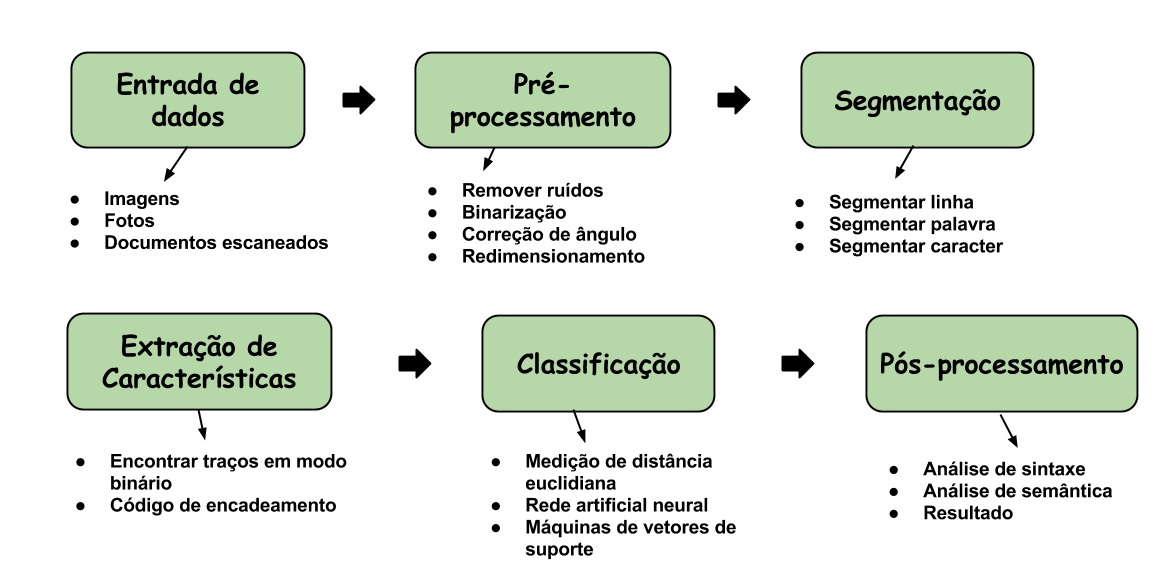
\includegraphics[width=.9\textwidth]{figuras/f3c2.png}
\end{center}
\legend{Fonte: o autor}
\end{figure}

As etapas ilustradas pela Figura 4 podem ser descritas da seguinte forma \cite{shah2013literature}:

\begin{alineas}
\item A etapa de entrada de dados é quando se adquire as imagens que serão analisadas, sejam fotografias, imagens coletadas de outras formas ou documentos escaneados. 
\item O pré-processamento é onde a imagem de entrada deve ser trabalhada para que esteja na melhor condição possível antes de chegar no ponto onde será segmentada. Isso envolve certos pontos importantes como a aplicação de \textit{filtros} utilizados em processamento de imagens como:
	\begin{subalineas}
		\item Remoção de ruídos: Erros de escaneamento, \textit{pixels} indesejados e problemas 			semelhantes são removidos ou tratados;
		\item Binarização (Limiarização): Processo que converte em preto e branco as imagens coloridas e que 	também ajuda no destacamento do caracter;
		\item Correção de ângulo: Adequa o ângulo para que os caracteres possam ser reconhecidos corretamente;
		\item Redimensionamento: Passo que auxilia principalmente em relação ao tempo de 					processamento.
	\end{subalineas} 
\item A segmentação é feita através de histogramas, dividida em duas partes, uma para identificar a linha onde estão as palavras e letras e outra para identificar colunas, separando caracter por caracter.
\item Extração de características é considerado o principal passo de extração de padrões em si. Dentro dessa fase encontram-se diversas técnicas, como a binarização, encadeamento dos resultados, histogramas dentre outros
\item A classificação recebe as informações da extração de características e com isto, mede a distância entre os pontos semelhantes e faz uma comparação com um padrão pré-armazenado que a própria OCR contém, buscando em que classe a informação recebida como entrada melhor se encaixa. A fórmula da distância entre os pontos \textit{euclidianos} será utilizada também em outras áreas no que diz respeito ao desenvolvimento deste projeto, e é dada por $ d(u , v) = |u - v| $ \cite{steinbruch1975algebra}.

\item O pós-processamento não é considerado como uma etapa essencial ou obrigatória. Porém pode ajudar num melhor resultado. Basicamente, trata de erros de caracteres muito parecidos, tais como a letra $O$ e o número $0$. 
\end{alineas}

As bibliotecas OCRs que serão usadas no desenvolvimento, providenciam a leitura OCR. Isso significa que elas são capazes de fazer as etapas de segmentação, extração de características e de classificação descritas no item b. As etapas de entrada de dados, pré-processamento e pós-processamento são necessárias para aumento da taxa de acerto, e serão realizadas através da biblioteca OpenCV em conjunto com o Python.

A \autoref{fig:filtros} representa os principais filtros usados na etapa de pré-processamento. O item (a) indica uma imagem original, o item (b) a imagem passada pelo processo de dilatação, o item(c) pelo processo de erosão, o item (d) pelo processo de maioria, o item (e) pelo processo de abertura e por fim o item (f) passa pelo processo de fechamento. Alguns destes processos serão utilizados posteriormente na sessão de desenvolvimento, consequentemente receberão um melhor detalhamento de como funcionam na prática \cite{caap}.

\begin{figure}[htbp]
\caption{\label{fig:filtros}Filtros de processamento de imagens aplicados a uma imagem}
\begin{center}
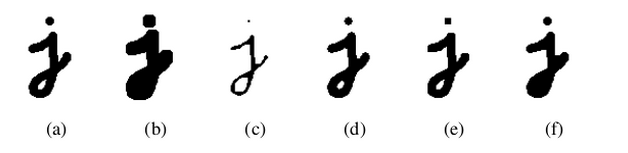
\includegraphics[width=.9\textwidth]{figuras/f4c2.png}
\end{center}
\legend{Fonte: \citeonline{caap}}
\end{figure}

\section{Conclusão}

Nesse capítulo foram apresentados conceitos fundamentais sobre visão computacional dando exemplos de onde se é aplicado. Também foi analisado os conceitos básicos de um sistema OCR. O próximo capítulo tem o objetivo de demonstrar certas ferramentas que serão aplicadas no capítulo de desenvolvimento.
